% ECSE 552 project presentation (20%): group 9, Wednesday December 2, 2026, 16:00-17:30.
% 15 min + 5 min Q/A; every member presents. PDF due on myCourses by November 29.
% Structure: docs/guidelines.md (storyline, the instructor's sample talk); B1--B8 and the
% rubric: docs/course-requirements.md. Numbers come from docs/experiments/ and the report;
% pending parts are red \todo and must stay visible until filled.
% Each slide: the section in the grey band (\topicsection), its main idea as the frame title.
\documentclass[aspectratio=169,11pt]{beamer}

\usepackage[utf8]{inputenc}
\usepackage[T1]{fontenc}
\usepackage{booktabs}
\usepackage{amsmath}
\usepackage{tikz}
\usetikzlibrary{arrows.meta,positioning,calc}

\usetheme{default}
\usefonttheme{professionalfonts}
\setbeamertemplate{navigation symbols}{}
\setbeamertemplate{footline}{\hfill\footnotesize\insertframenumber\,/\,\inserttotalframenumber\hspace{1em}\vspace{0.6em}}
\setbeamersize{text margin left=0.7cm, text margin right=0.7cm}
\setbeamertemplate{itemize items}[circle]
\definecolor{accent}{RGB}{0,84,147}
\setbeamercolor{structure}{fg=accent}
\setbeamercolor{frametitle}{fg=accent}
\setbeamercolor{topic}{bg=gray!14, fg=gray!60!black}
\setbeamerfont{topic}{series=\bfseries, size=\Large}
\setbeamerfont{frametitle}{series=\bfseries, size=\large}

% Section name in a grey band; the frame title below it is the slide's main idea.
\def\topicname{}
\newcommand{\topic}[1]{\gdef\topicname{#1}}
\newcommand{\topicsection}[1]{\section{#1}\topic{#1}}
\setbeamertemplate{frametitle}{%
  \nointerlineskip
  \begin{beamercolorbox}[wd=\paperwidth, ht=0.62cm, dp=0.22cm, leftskip=0.7cm]{topic}
    \usebeamerfont{topic}\topicname
  \end{beamercolorbox}\par
  \vskip0.18cm
  \begin{beamercolorbox}[wd=\paperwidth, leftskip=0.7cm, rightskip=0.7cm plus 1fil]{frametitle}
    \usebeamerfont{frametitle}\insertframetitle
  \end{beamercolorbox}}

\newcommand{\todo}[1]{\textcolor{red}{[TODO: #1]}}
\newcommand{\src}[1]{\vfill{\scriptsize\color{gray}#1}}
% Opens the video next to the PDF (docs/presentation/videos/); the frames stay in the PDF.
\newcommand{\play}[1]{\href{run:videos/#1.mp4}{\beamerbutton{$\blacktriangleright$ Video}}}
\newcommand{\strip}[1]{\includegraphics[width=\linewidth]{figures/strip_#1.png}}
\newcommand{\step}[1]{\textcolor{red}{Step #1:}}
\newcommand{\fix}{\textcolor{red}{$\rightarrow$}}

% Diagrams: the colours of the result charts (IDM purple as (b), DANN magenta as (c), ACT
% blue); data grey, solid with actions and dashed for videos without actions. One box size
% per diagram, thin outlines and arrows of one style.
\definecolor{cidm}{HTML}{7C4DBD}
\definecolor{cdann}{HTML}{D55181}
\definecolor{cact}{HTML}{2A78D6}
\tikzset{
  box/.style={draw, line width=0.7pt, rounded corners=3pt, align=center, text width=2.4cm,
    minimum height=1cm, font=\scriptsize},
  data/.style={box, draw=black!55, fill=black!5},
  video/.style={data, dashed},
  idm/.style={box, draw=cidm, fill=cidm!12},
  dann/.style={box, draw=cdann, fill=cdann!12},
  policy/.style={box, draw=cact, fill=cact!12},
  arr/.style={-{Latex[length=1.8mm]}, line width=0.7pt, draw=black!75}}

% The method, one slide per step: the steps so far (earlier ones grey) and the pipeline,
% whose later boxes are kept in place but hidden until their step.
\newcommand{\stepone}{train an IDM on the source demos; for (c), with DANN on target frames.}
\newcommand{\steptwo}{label every target video; drop videos whose labels jump over 2~rad.}
\newcommand{\stepthree}{train ACT on the source demos plus the labeled videos.}
\newcommand{\steps}[1]{\begin{minipage}[t][1.15cm][t]{\linewidth}\vspace{0pt}\footnotesize\raggedright
  \ifnum#1=1 \step{1} \stepone\par\else{\color{gray}Step 1: \stepone}\par\fi
  \ifnum#1=2 \step{2} \steptwo\par\fi
  \ifnum#1>2 {\color{gray}Step 2: \steptwo}\par\fi
  \ifnum#1=3 \step{3} \stepthree\par\fi
  \end{minipage}}
\newcommand{\pipeline}[1]{%
  \begin{tikzpicture}[node distance=0.7cm and 0.7cm, scale=0.82, transform shape]
    \tikzset{s2/.style={}, s3/.style={}}
    \ifnum#1<2 \tikzset{s2/.style={opacity=0, text opacity=0}}\fi
    \ifnum#1<3 \tikzset{s3/.style={opacity=0, text opacity=0}}\fi
    \node[data] (src) {Source demos\\images + actions};
    \node[idm, right=of src] (idm) {\textbf{1.} IDM\\$\hat{a}_t = f_\theta(o_t, o_{t+1})$};
    \node[data, s2, right=of idm] (pl) {\textbf{2.} Target videos\\with pseudo-labels};
    \node[policy, s3, right=of pl] (act) {\textbf{3.} ACT policy\\images only};
    \node[video, below=of src] (tgt) {Target videos\\images only};
    \node[dann, below=of idm] (dann) {DANN (c)\\discriminator};
    \draw[arr] (src) -- (idm);
    \draw[arr] (tgt) -- (dann);
    \draw[arr, <->] (dann) -- (idm);
    \draw[arr, s2] (idm) -- (pl);
    \draw[arr, s2] (tgt.south) -- ++(0,-0.35) -| (pl.south);
    \draw[arr, s3] (pl) -- (act);
    \draw[arr, s3] (src.north) -- ++(0,0.35) -| (act.north);
  \end{tikzpicture}}

\title{Learning to Manipulate a New Object\\from Action-Free Videos}
\author{Group 9: Brik Meza, Gonzalo Mill\'an Garc\'ia, Myriam Dardour, Zheng Ye Zhang}
\institute{McGill University --- ECSE 552 Deep Learning}
\date{December 2, 2026}

\begin{document}

\begin{frame}[plain]
  \titlepage
\end{frame}

\topic{Outline}
\begin{frame}{From the problem to what worked and what did not}
  \tableofcontents
\end{frame}

% ================================================================ Motivation (B1--B3)
% Presenter (proposed): Brik, slides 3--7.
\topicsection{Motivation}

\begin{frame}{Every new task needs new demonstrations, and they are expensive}
  \begin{columns}[c]
    \begin{column}{0.48\textwidth}
      \begin{itemize}
        \item Policies such as ACT imitate images paired with motor commands.
        \item A new task or object means new teleoperated demos (right).
        \item DROID: 76k demos, 50 people, one year.
      \end{itemize}
    \end{column}
    \begin{column}{0.5\textwidth}
      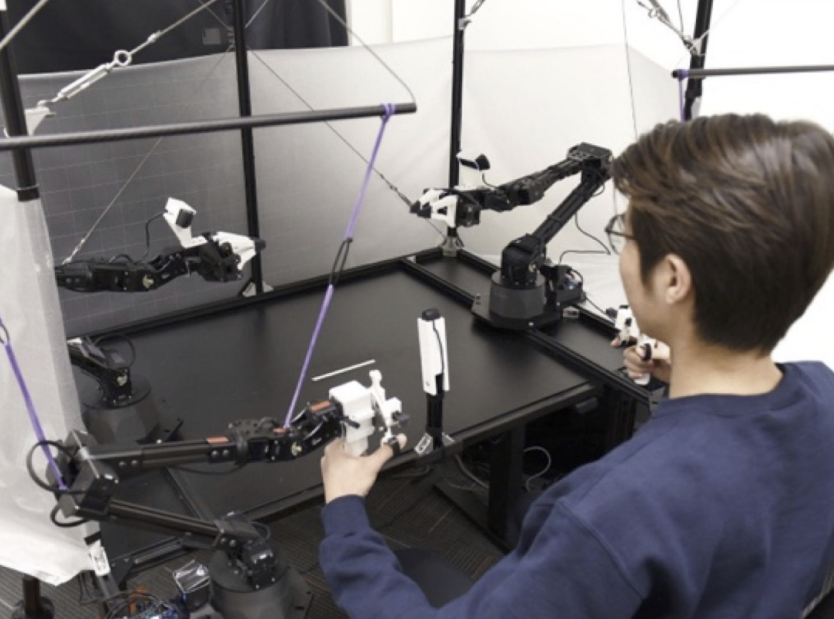
\includegraphics[width=\linewidth]{figures/aloha.png}\\[1pt]
      {\scriptsize Teleoperation with ALOHA. Photo: Zhao et al.\ (2023).}
    \end{column}
  \end{columns}
  \src{Zhao et al.\ 2023 (ALOHA, ACT); Chi et al.\ 2023; Khazatsky et al.\ 2024 (DROID)}
\end{frame}

\begin{frame}{Generative video models can produce demonstrations, but without actions}
  \begin{columns}[c]
    \begin{column}{0.48\textwidth}
      \centering
      \begin{tikzpicture}
        \node[draw=gray, dashed, minimum width=\linewidth, minimum height=4.2cm,
          text width=0.8\linewidth, align=center]
          {\todo{frames of a robot video made by a video generation model, with its
          citation}};
      \end{tikzpicture}
    \end{column}
    \begin{column}{0.5\textwidth}
      \begin{itemize}
        \item Video generation models are improving quickly and can produce robot videos.
          \todo{examples and citations}
        \item A generated video has images only, no motor commands to imitate.
        \item DreamGen labels generated videos with an inverse dynamics model.
      \end{itemize}
      \vspace{0.4em}
      \textbf{Question:} can a policy learn a new object from videos without actions?
    \end{column}
  \end{columns}
  \src{Jang et al.\ 2025 (DreamGen)}
\end{frame}

\begin{frame}{Application: a UR5e arm places an object in a goal square}
  \centering
  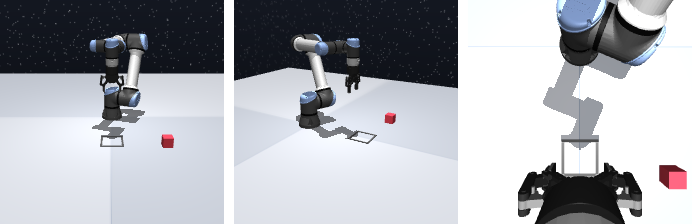
\includegraphics[width=0.6\linewidth]{figures/cameras.png}\\[1pt]
  {\scriptsize Front, side and wrist cameras, $224 \times 224$ at 10~Hz: the policy's only
  input.}\\[6pt]
  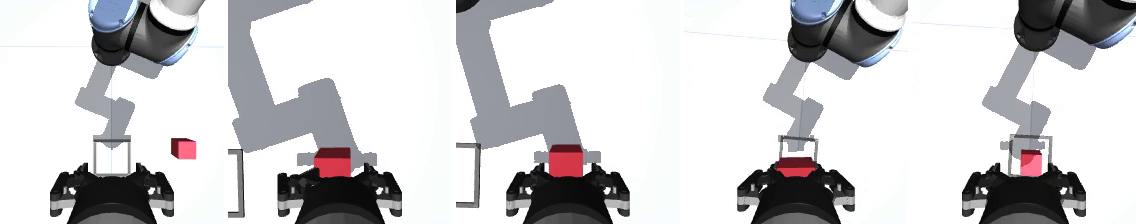
\includegraphics[width=0.6\linewidth]{figures/strip_a_source.png}\\[1pt]
  {\scriptsize Success: the whole object inside the 12~cm square, released and still,
  within 20~s. Source-only policy on the source cube (90.7\%). \play{task}}
  \src{OCBench: Park and Levine 2026}
\end{frame}

% Problem and constraints (B2, B3), still in the Motivation section.

\begin{frame}{Labels exist for the source object; the target has only videos}
  \begin{columns}[c]
    \begin{column}{0.4\textwidth}
      \centering
      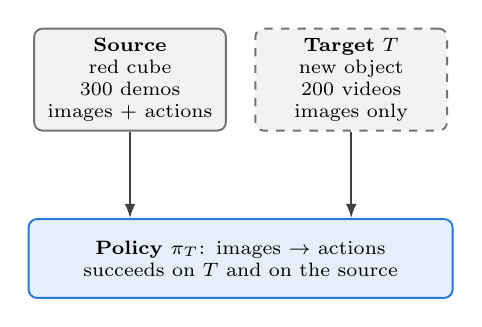
\begin{tikzpicture}[node distance=1.1cm and 0.35cm, box/.append style={text width=2.2cm}]
        \node[data] (s) {\textbf{Source}\\red cube\\300 demos\\images + actions};
        \node[video, right=of s] (t) {\textbf{Target} $T$\\new object\\200 videos\\images only};
        \node[policy, text width=5.15cm, below=1.1cm of $(s.south)!0.5!(t.south)$]
          (p) {\textbf{Policy} $\pi_T$: images $\rightarrow$ actions\\succeeds on $T$ and on the
          source};
        \draw[arr] (s.south) -- (s.south |- p.north);
        \draw[arr] (t.south) -- (t.south |- p.north);
      \end{tikzpicture}
      \[
        G_T = \frac{s(\pi_T, T) - s(\pi_a, T)}{s(\pi_d, T) - s(\pi_a, T)}
      \]
      {\scriptsize $s$: success; $\pi_a$: source only; $\pi_d$: oracle with true target
      actions.}
    \end{column}
    \begin{column}{0.58\textwidth}
      \scriptsize
      \begin{tabular}{@{}llp{3.3cm}l@{}}
        \toprule
        & Requirement & Definition & Target \\
        \midrule
        R1 & Supervision & Target data: frames only & No labels \\
        R2 & Label budget & Same source demos for all & 300 \\
        R3 & Inputs & No simulator state & Images only \\
        R4 & Target & Share of the oracle's gain & $G_T \geq 0.5$ \\
        R5 & Retention & Drop in source success & $\leq 10$ points \\
        R6 & Real time & Inference per 10~Hz step & $< 100$~ms \\
        \bottomrule
      \end{tabular}
    \end{column}
  \end{columns}
\end{frame}

% ================================================================ Related work
\topicsection{Related work}

\begin{frame}{\todo{main idea of the slide}}
  % To be researched by a team member: how policies learn from action-free videos.
  \todo{Existing approaches to learning from action-free videos, each with its shortcoming
  for a new object (as in the instructor's sample talk), with citations; then our idea in
  one sentence.}
\end{frame}

% ================================================================ Data (B6)
\topicsection{Data}

\begin{frame}{One source object and five targets, generated in simulation}
  \centering
  \begin{tikzpicture}
    \node[inner sep=0] (img) {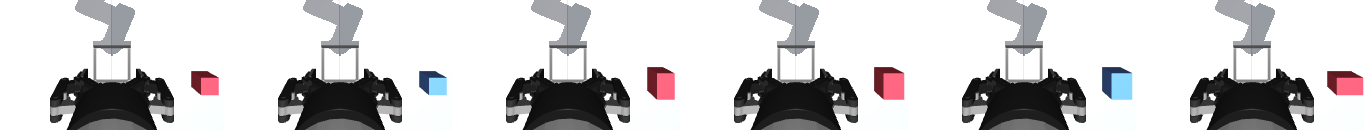
\includegraphics[width=0.85\linewidth]{figures/objects.png}};
    % Panel centres measured in objects.png.
    \foreach \x/\name in {0.098/Source, 0.265/A, 0.432/B, 0.600/C, 0.767/D, 0.935/E}
      \node[font=\scriptsize, below=1pt] at ($(img.south west)!\x!(img.south east)$) {\name};
  \end{tikzpicture}
  \vspace{0.3em}

  \scriptsize
  \begin{tabular}{@{}llllr@{}}
    \toprule
    Object & Shape (cm), colour & Change & Used by & Episodes \\
    \midrule
    Source & $6 \times 6 \times 6$, red & -- & Every policy, IDM & 300 \\
    Source, turned & $6 \times 6 \times 6$, red & -- & IDM only & 100 \\
    A & $6 \times 6 \times 6$, blue & Appearance & Videos (b, c); actions (d) & 200 \\
    B & $9 \times 6 \times 6$, red & Geometry & As A & 200 \\
    C & $9 \times 7 \times 6$, red & Geometry, grasp width & As A & 200 \\
    D & $9 \times 7 \times 6$, blue & All three & As A & 200 \\
    E & $6 \times 9 \times 6$, red & \textbf{Behaviour}: turned grasp & As A & 200 \\
    \bottomrule
  \end{tabular}\\[3pt]
  Start uniform in a $20 \times 20$~cm area, yaw 0; same initial states for every object;
  scripted expert, 94--100\% success.
\end{frame}

% ================================================================ Method (B4, B5)
% Presenter (proposed): Zheng Ye, slides 8--10.
\topicsection{Method}

\begin{frame}[t]{Step 1: an IDM learns the action between two frames from the source}
  \steps{1}
  \centering
  \pipeline{1}\\[4pt]
  \begin{minipage}{0.28\linewidth}
    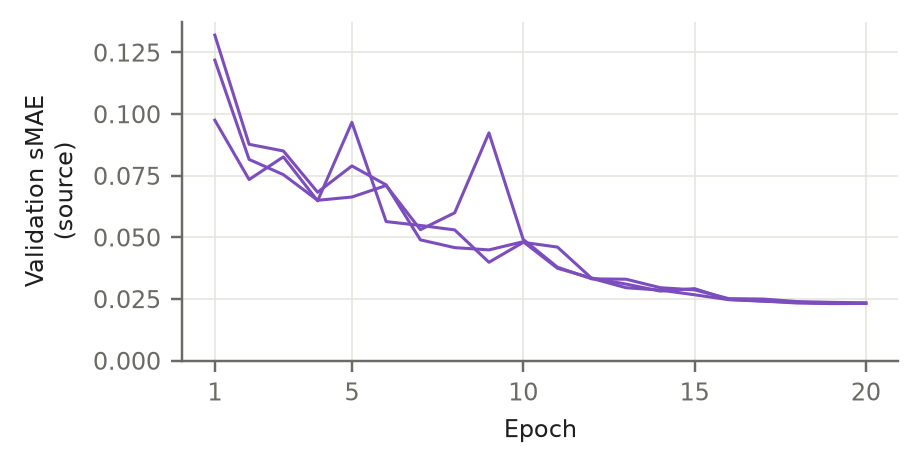
\includegraphics[width=\linewidth]{../report/figures/idm_val.png}
  \end{minipage}\hspace{0.5em}%
  \begin{minipage}{0.3\linewidth}
    \scriptsize Validation error of the IDM on held-out source transitions, per epoch,
    three seeds: 0.023 at the end.
  \end{minipage}
\end{frame}

\begin{frame}{The IDM reads the action from the motion between two frames}
  \centering
  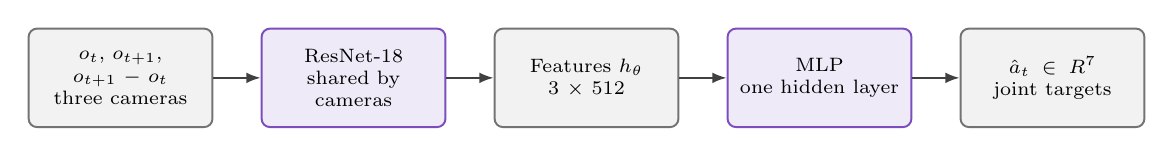
\begin{tikzpicture}[node distance=0.6cm, box/.append style={text width=2.1cm, minimum height=1.25cm}]
    \node[data] (in) {$o_t$, $o_{t+1}$, $o_{t+1} - o_t$\\three cameras};
    \node[idm, right=of in] (enc) {ResNet-18\\shared by cameras};
    \node[data, right=of enc] (h) {Features $h_\theta$\\$3 \times 512$};
    \node[idm, right=of h] (mlp) {MLP\\one hidden layer};
    \node[data, right=of mlp] (a) {$\hat{a}_t \in \mathbb{R}^7$\\joint targets};
    \draw[arr] (in) -- (enc);
    \draw[arr] (enc) -- (h);
    \draw[arr] (h) -- (mlp);
    \draw[arr] (mlp) -- (a);
  \end{tikzpicture}\\[4pt]
  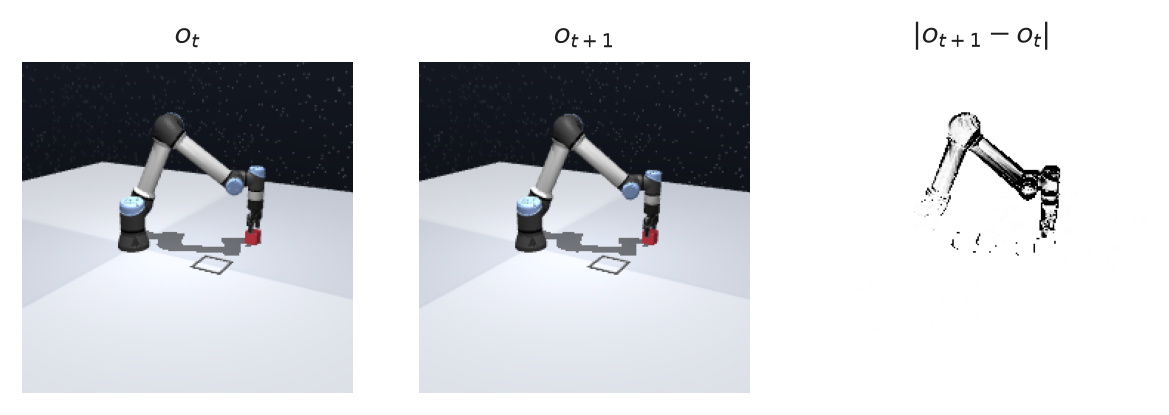
\includegraphics[width=0.62\linewidth]{../report/figures/idm_input.png}\\
  \raggedright\small
  \begin{itemize}
    \item The difference keeps the motion and drops static appearance such as colour.
    \item Trained on 300 source demos + 100 with a turned grasp; one IDM for every target.
  \end{itemize}
  \src{Torabi et al.\ 2018; Baker et al.\ 2022; Morin et al.\ 2026}
\end{frame}

% Presenter (proposed): Myriam, DANN.
\begin{frame}{For (c), DANN pushes the IDM to features that hide the domain}
  \centering
  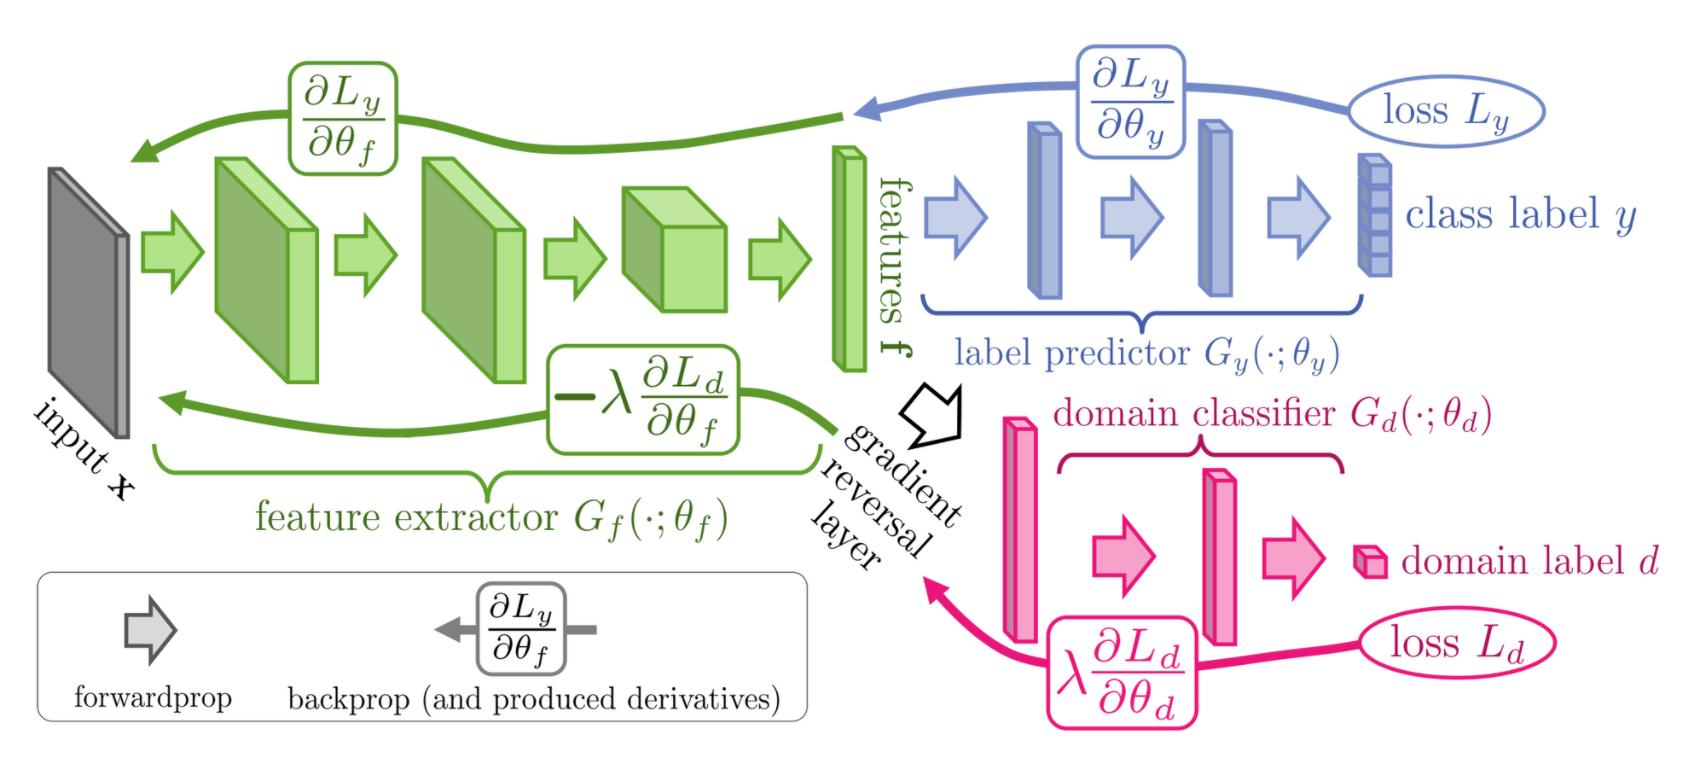
\includegraphics[width=0.66\linewidth]{figures/dann_ganin.png}\\[2pt]
  \raggedright\small
  \begin{itemize}
    \item Ours: $G_f$ is the IDM's ResNet-18; $G_y$ regresses the action (MSE, not a
      class); $G_d$ is an MLP $1536 \rightarrow 256 \rightarrow 1$.
    \item Each step: 64 source + 64 target pairs; $\lambda$ ramps to 0.5; fixed before any
      run. Control: $\lambda = 0$.
  \end{itemize}
  \src{Figure: Ganin et al.\ 2016}
\end{frame}

\begin{frame}[t]{Step 2: the IDM labels every target video; impossible labels are dropped}
  \steps{2}
  \centering
  \pipeline{2}\\[4pt]
  \begin{minipage}{0.42\linewidth}
    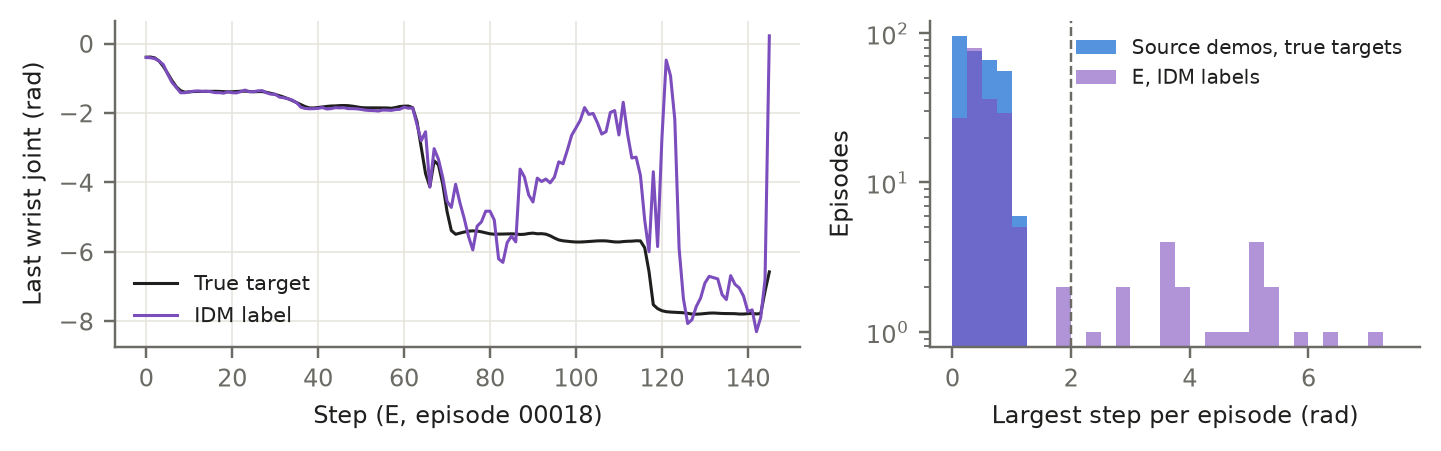
\includegraphics[width=\linewidth]{../report/figures/labels.png}
  \end{minipage}\hspace{0.5em}%
  \begin{minipage}{0.3\linewidth}
    \scriptsize Wrist labels against the truth on one E video, and the largest step per
    episode: the source demos never step over 1.1~rad.
  \end{minipage}
\end{frame}

\begin{frame}[t]{Step 3: ACT trains on the source demos plus the labeled videos}
  \steps{3}
  \centering
  \pipeline{3}
  \vspace{0.6em}

  \raggedright
  \textbf{Hypothesis:} (c) gives better labels and higher success than (b).
\end{frame}

\begin{frame}{ACT stays fixed; the methods change its training data}
  \centering
  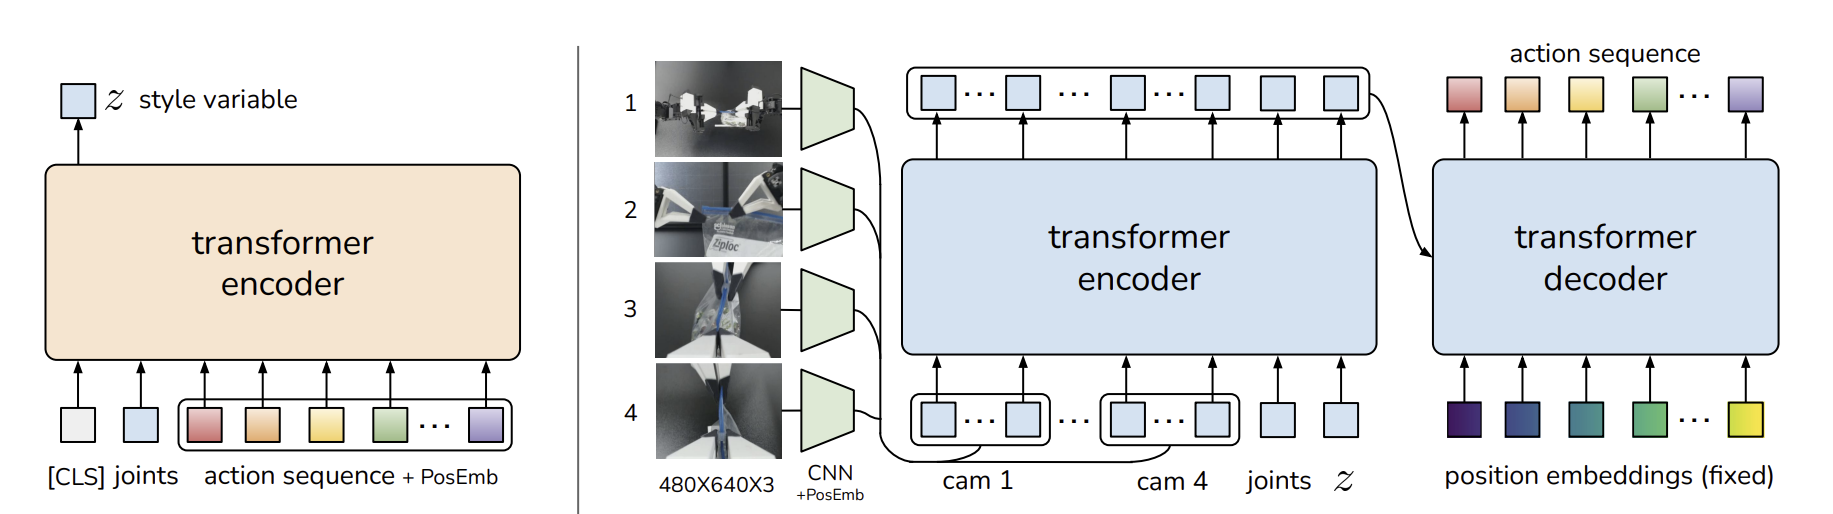
\includegraphics[width=0.74\linewidth]{figures/act.png}\\[1pt]
  {\scriptsize Ours: 3 cameras at $224 \times 224$, joints set to zero (R3), chunks of 20
  joint targets, $z = 0$ at test; original code and settings unchanged.\par}
  \vspace{0.4em}

  \scriptsize\setlength{\tabcolsep}{4pt}
  \begin{tabular}{@{}lllll@{}}
    \toprule
    & Method & What is trained & ACT trains on & What changes vs.\ (a) \\
    \midrule
    (a) & Source only & ACT & 300 source demos & Nothing (reference) \\
    (e) & Augmentation & ACT & 300 source demos, colour jitter & The training images \\
    (d) & Oracle & ACT & + 200 target demos, true actions & True target actions \\
    (b) & Unadapted IDM & IDM, then ACT & + 200 target videos, IDM labels & IDM labels the videos \\
    (c) & DANN-adapted IDM & IDM + discriminator, ACT & + 200 target videos, its labels &
      How the IDM trains \\
    \bottomrule
  \end{tabular}
  \src{Figure: Zhao et al.\ 2023}
\end{frame}

% ================================================================ Evaluation
\topicsection{Evaluation}

\begin{frame}{Every number comes from closed-loop rollouts on reserved seeds}
  \centering
  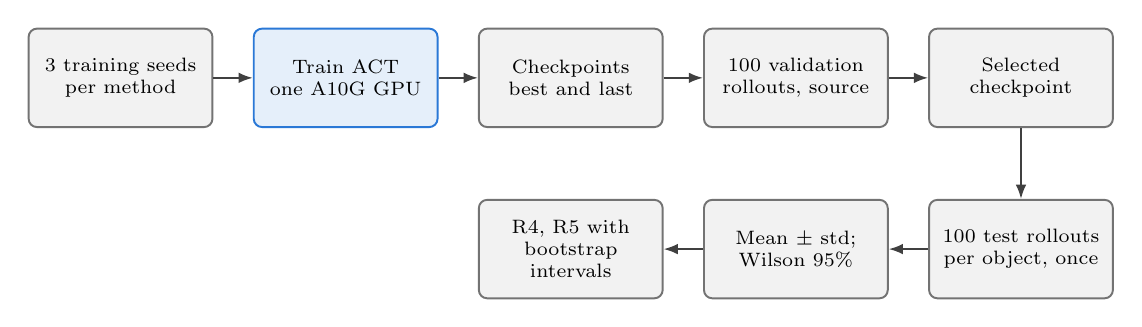
\begin{tikzpicture}[node distance=0.9cm and 0.5cm, box/.append style={text width=2.1cm, minimum height=1.25cm}]
    \node[data] (seeds) {3 training seeds\\per method};
    \node[policy, right=of seeds] (train) {Train ACT\\one A10G GPU};
    \node[data, right=of train] (ckpt) {Checkpoints\\best and last};
    \node[data, right=of ckpt] (val) {100 validation\\rollouts, source};
    \node[data, right=of val] (sel) {Selected\\checkpoint};
    \node[data, below=of sel] (test) {100 test rollouts\\per object, once};
    \node[data, below=of val] (stats) {Mean $\pm$ std;\\Wilson 95\%};
    \node[data, below=of ckpt] (req) {R4, R5 with\\bootstrap intervals};
    \draw[arr] (seeds) -- (train);
    \draw[arr] (train) -- (ckpt);
    \draw[arr] (ckpt) -- (val);
    \draw[arr] (val) -- (sel);
    \draw[arr] (sel) -- (test);
    \draw[arr] (test) -- (stats);
    \draw[arr] (stats) -- (req);
  \end{tikzpicture}
  \vspace{0.6em}

  \raggedright\small
  \begin{itemize}
    \item Reserved seeds: validation rollouts from 900,000, test rollouts from 1,000,000;
      the same initial states for every method.
    \item Target actions only for the oracle and the label error (R1).
    \item Splits: ACT 80/20 by episode; IDM 8 of every 10; DANN adapts on 160 of 200
      target videos.
  \end{itemize}
\end{frame}

\begin{frame}{Validation loss does not tell which checkpoint succeeds}
  \centering
  \begin{columns}[c]
    \begin{column}{0.49\textwidth}
      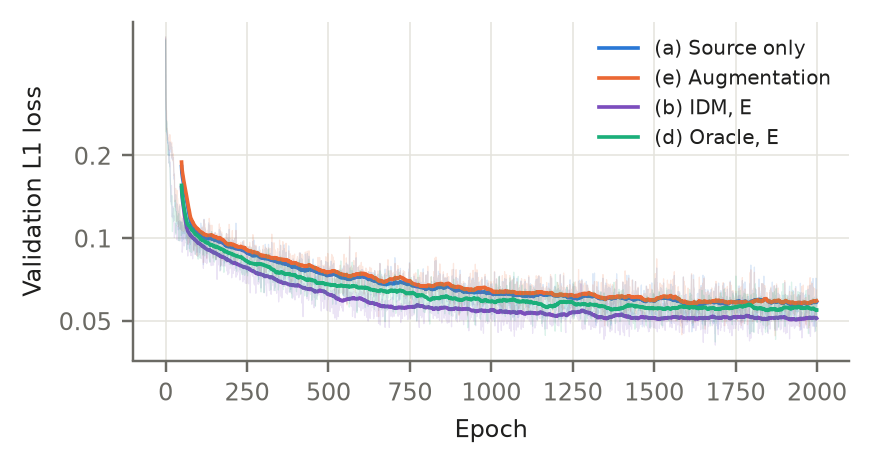
\includegraphics[width=\linewidth]{../report/figures/act_val.png}\\
      {\scriptsize ACT validation loss per epoch, seed 0 (50-epoch moving average).}
    \end{column}
    \begin{column}{0.49\textwidth}
      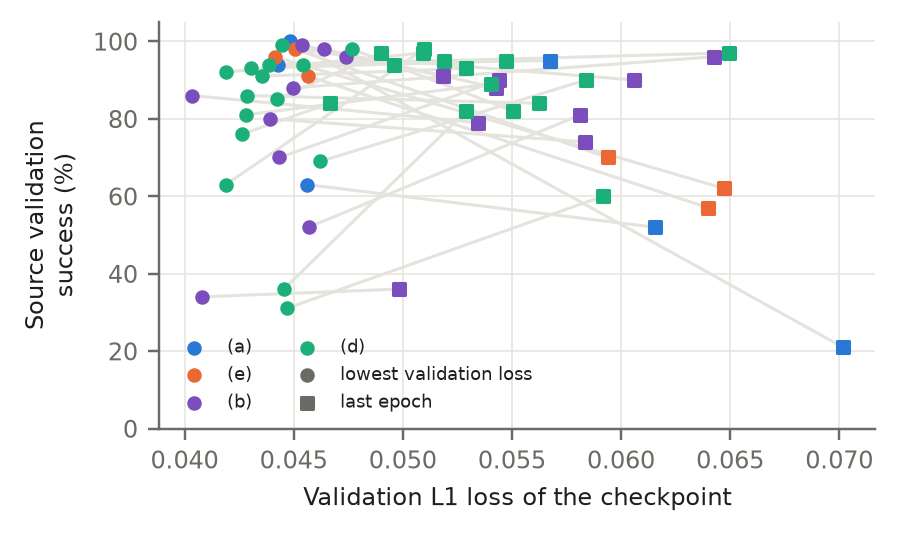
\includegraphics[width=\linewidth]{../report/figures/act_selection.png}\\
      {\scriptsize Two checkpoints per run, 30 runs: lower loss, not higher success.}
    \end{column}
  \end{columns}
  \vspace{0.6em}

  \raggedright\small
  The checkpoint is chosen by 100 source validation rollouts: \emph{last} 17 times,
  \emph{lowest loss} 13 times, up to 79 points apart.
\end{frame}

% ================================================================ Results (B7)
% Presenter (proposed): Gonzalo, slides 13--14.
\topicsection{Results}

\begin{frame}{Appearance needs no target videos; behaviour does}
  \begin{columns}[c]
    \begin{column}{0.5\textwidth}
      \footnotesize
      (e) Colour jitter, no target data, on the blue cube A: \textbf{98.7\%}\\[1pt]
      \strip{e_A}\\[1pt]
      \hfill\play{appearance}\\[3pt]
      The same kind of policy on block E: \textbf{0.3\%}\\[1pt]
      \strip{e_E}\\[1pt]
      \hfill\play{behaviour}
    \end{column}
    \begin{column}{0.46\textwidth}
      \footnotesize
      \centering
      \begin{tabular}{@{}lrr@{}}
        \toprule
        Policy & A & E \\
        \midrule
        (a) Source only & 0.3\% & 0\% \\
        (e) Augmentation & \textbf{98.7\%} & 0.3\% \\
        (a) + 100 turned demos & -- & 2.3\% \\
        (d) Oracle & 85.7\% & \textbf{89.0\%} \\
        \bottomrule
      \end{tabular}\\[6pt]
      \raggedright
      E's 9~cm side does not fit the 8.5~cm gripper: the grasp must turn by $90^\circ$,
      and \emph{when} to turn is only in E's videos.
    \end{column}
  \end{columns}
\end{frame}

\begin{frame}{Target videos pay off where augmentation cannot}
  \centering
  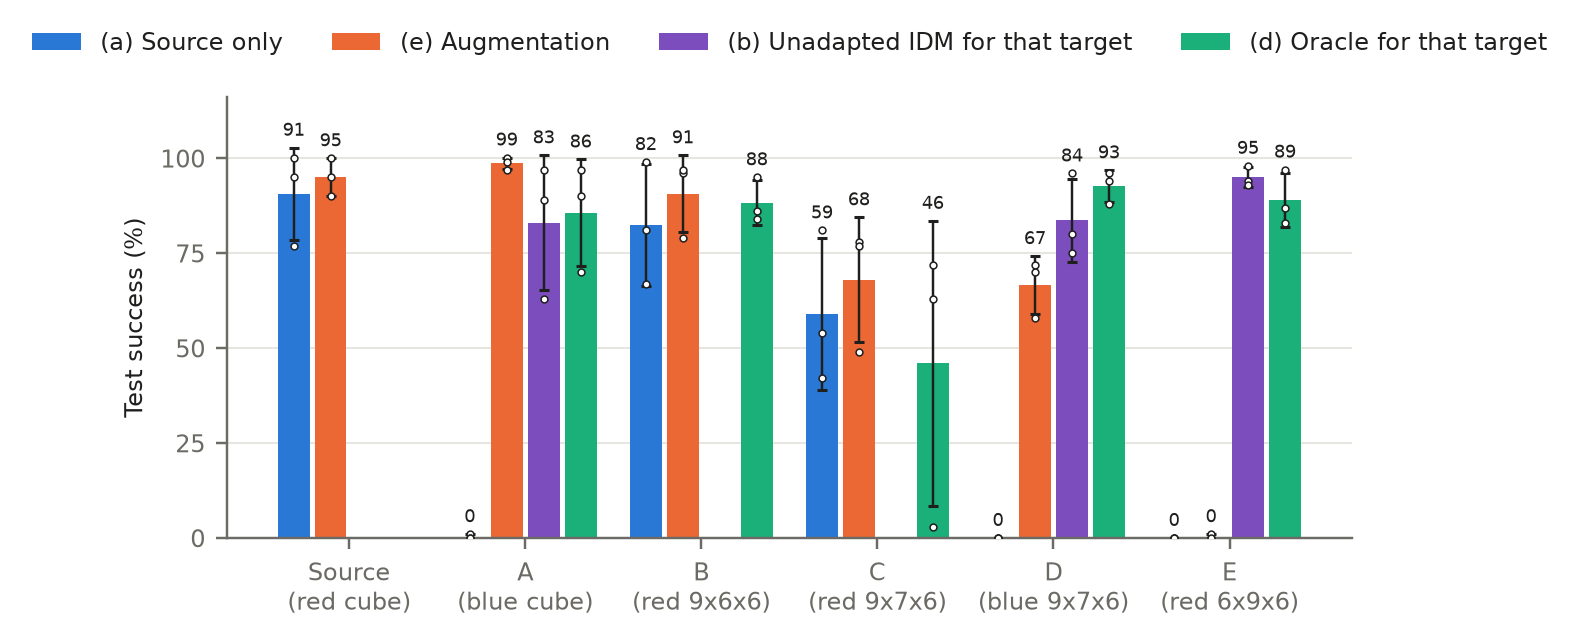
\includegraphics[width=0.86\linewidth]{../report/figures/results.png}
  \raggedright\small
  \begin{itemize}
    \item (b) meets R4 on A, D, E: $G_T$ = 0.97 [0.73, 1.25], 0.90 [0.79, 1.04], 1.07
      [0.98, 1.17].
    \item (c), seed 0: 6\%, 0\%, 0\% on A, D, E, the level of (a). Its labels are worse
      than (b)'s on every target.
  \end{itemize}
\end{frame}

% Presenter (proposed): Brik, slide 15.
\begin{frame}{The videos of E teach the policy when to turn}
  \begin{columns}[c]
    \begin{column}{0.5\textwidth}
      \footnotesize
      (e) Augmentation, on block E: \textbf{0.3\%}\\[1pt]
      \strip{e_E}\\[4pt]
      (b) IDM pseudo-labels from E's videos: \textbf{95.0\%}\\[1pt]
      \strip{b_E}\\[2pt]
      \hfill\play{idm}
    \end{column}
    \begin{column}{0.47\textwidth}
      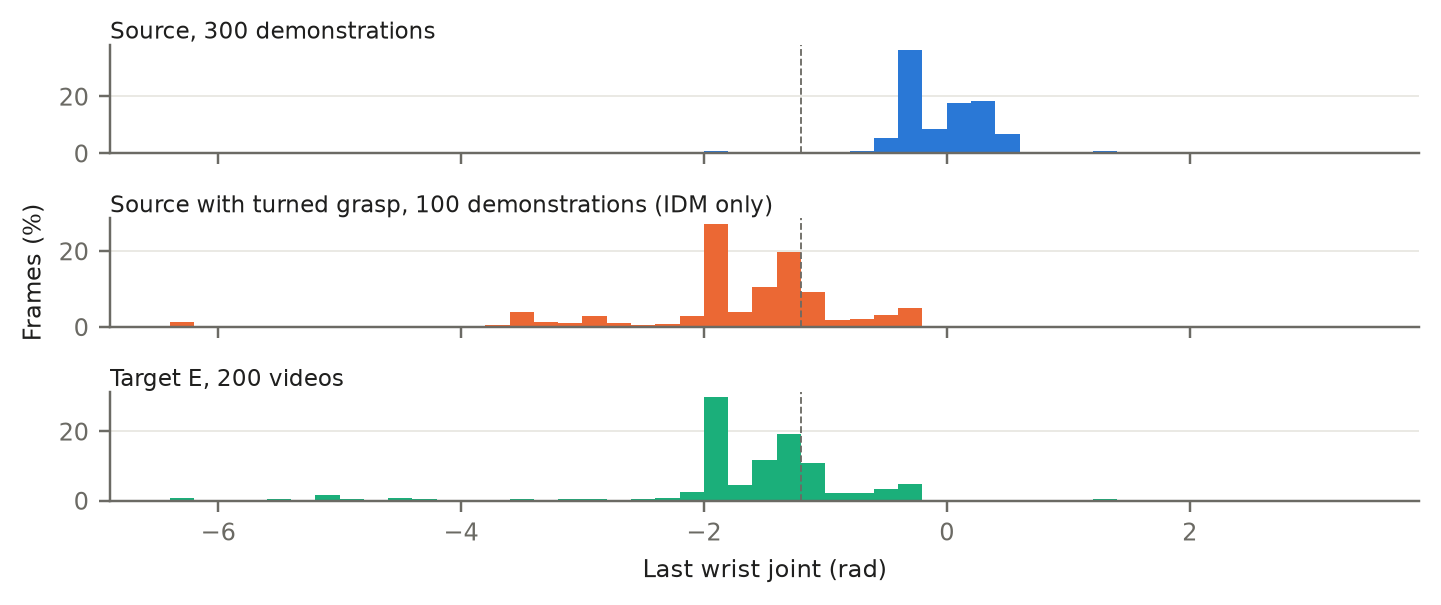
\includegraphics[width=\linewidth]{../report/figures/wrist.png}\\
      \scriptsize E needs wrist angles that are rare in the source demos; the 100 turned
      source demos give the IDM those motions.
    \end{column}
  \end{columns}
  \vspace{0.3em}
  \begin{itemize}
    \small
    \item Full-turn wrist errors: the filter drops them (about 10\% of E); same success
      without it.
  \end{itemize}
\end{frame}

% Presenter (proposed): Myriam, slide 16.
\begin{frame}{Adapting the IDM with DANN makes the labels worse}
  \centering
  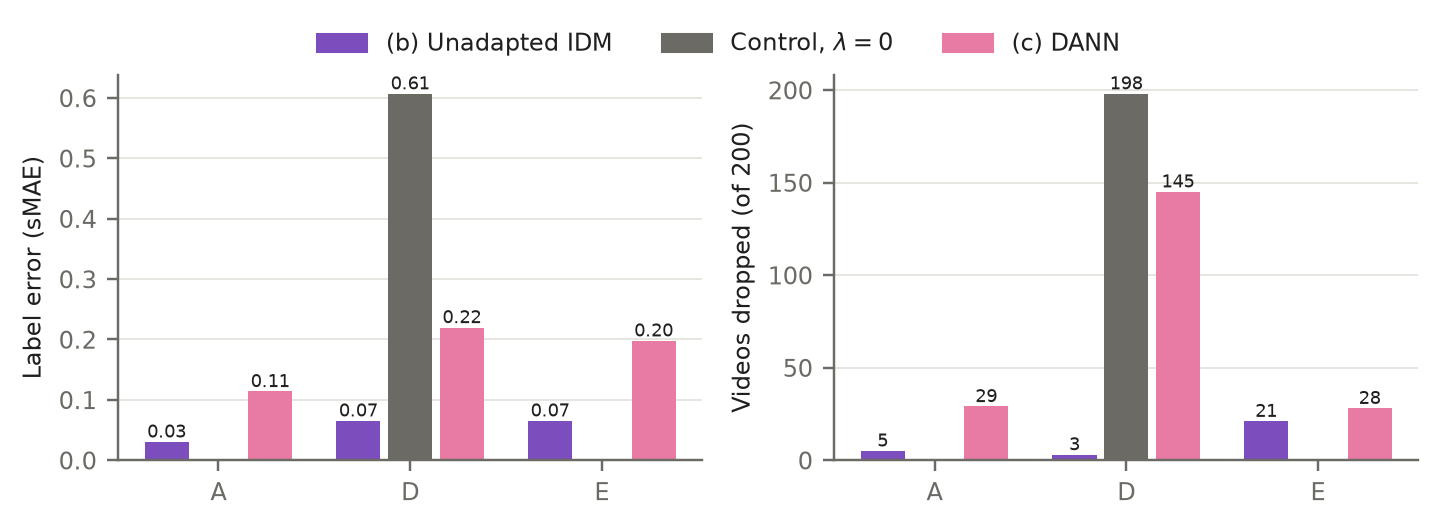
\includegraphics[width=0.84\linewidth]{../report/figures/dann.png}
  \raggedright\small
  \begin{itemize}
    \item One seed (0); rule fixed before measuring: 5\% below (b)'s best seed.
    \item DANN: 3--4$\times$ (b)'s error on A, D, E, mostly the wrist, in every phase: a
      constant offset ($-0.7$~rad on D), not full turns, so the filter keeps it.
    \item Control ($\lambda = 0$) worst: 0.607 on D. Target images in the batches change
      the weights, not the batch-norm statistics.
    \item The rule stops (c) here; we still trained its policies on seed 0: 6\%, 0\%, 0\%,
      the object lifted in 5 of 150 validation rollouts.
  \end{itemize}
  \src{Label error against the true actions, for evaluation only (R1).}
\end{frame}

% ================================================================ Critique (B8)
% Presenter (proposed): Brik, slides 17--18.
\topicsection{Critique}

\begin{frame}{The constraints hold for (b); most problems led to a fix}
  \begin{columns}[T]
    \begin{column}{0.47\textwidth}
      \footnotesize
      \begin{tabular}{@{}lp{4.8cm}@{}}
        \toprule
        R1, R3 & Met by design \\
        R2 & 300 demos (100 reach 37\%) \\
        R4 & (e): A, B, D. (b): A, D, E. (c), seed 0: none \\
        R5 & (e) and (b) on A, D. Not (b) on E: one seed. (c), seed 0: A, D \\
        R6 & Met: 10--18~ms per call \\
        \bottomrule
      \end{tabular}
    \end{column}
    \begin{column}{0.51\textwidth}
      \footnotesize
      \begin{itemize}
        \item Own ACT at 23--49\% \fix{} the original ACT.
        \item First targets solved by jitter \fix{} target E.
        \item IDM could not label E \fix{} 100 turned source demos.
        \item Full-turn wrist errors \fix{} a 2~rad label filter.
        \item DANN made labels worse \fix{} reported as negative transfer.
        \item High seed variance \fix{} 3 seeds, rollout selection, intervals.
      \end{itemize}
    \end{column}
  \end{columns}
\end{frame}

% ================================================================ Conclusions (B8)
\topicsection{Conclusions}

\begin{frame}{Videos help when the behaviour changes; adapting the IDM did not}
  \begin{columns}[T]
    \begin{column}{0.5\textwidth}
      \textbf{Conclusions}
      \begin{enumerate}
        \footnotesize
        \item Augmentation covers appearance; videos are needed for a new behaviour.
        \item IDM-labeled videos recover 0.90 (D) and 1.07 (E) of the oracle's gain.
        \item The IDM must have seen the motion in source data.
        \item DANN made the labels worse; its policies (c) fail as (a).
        \item No target labels; ACT unchanged, 15~ms per call.
      \end{enumerate}
    \end{column}
    \begin{column}{0.48\textwidth}
      \textbf{Limitations}
      \begin{itemize}
        \footnotesize
        \item Simulation, one task \fix{} real or human videos.
        \item Fixed yaw and start \fix{} stock OCBench.
        \item Three seeds \fix{} more seeds.
        \item IDM sees source motions only \fix{} iterative BCO. \todo{run or future work}
        \item DANN aligns whole distributions \fix{} regression-aware alignment.
      \end{itemize}
    \end{column}
  \end{columns}
\end{frame}

\topic{Questions}
\begin{frame}{Thank you}
  \centering
  \vspace{1.2em}
  {\Huge Questions?}
  \vspace{2em}

  \raggedright\small
  \begin{tabular}{@{}ll@{}}
    Code & \url{https://github.com/BrikHMP18/ecse-552-project} \\
    Data & \url{https://huggingface.co/datasets/Autobrik/ecse552-ocbench-block} \\
    Models & \url{https://huggingface.co/Autobrik} (\texttt{ecse552-act-*}) \\
  \end{tabular}
\end{frame}

% ---------------------------------------------------------------- Backup (Q/A)
\appendix
\topic{Backup}

\begin{frame}{R4 and R5 with 95\% intervals}
  \centering
  \small
  \begin{tabular}{@{}llrlrl@{}}
    \toprule
    Target & Method & $G_T$ & Interval & Source drop & Interval \\
    \midrule
    A & (e) & 1.15 & [1.02, 1.40] & $-4.3$ & [$-18.0$, 7.0] \\
    A & (b) & 0.97 & [0.73, 1.25] & $-2.0$ & [$-15.3$, 9.0] \\
    D & (e) & 0.72 & [0.62, 0.82] & $-4.3$ & [$-18.0$, 7.0] \\
    D & (b) & 0.90 & [0.79, 1.04] & $-2.7$ & [$-15.7$, 7.7] \\
    E & (e) & 0.00 & [0.00, 0.02] & $-4.3$ & [$-17.7$, 7.0] \\
    E & (b) & 1.07 & [0.98, 1.17] & 19.7 & [$-3.7$, 46.3] \\
    \bottomrule
  \end{tabular}

  \vspace{0.5em}
  Bootstrap: training seeds with replacement, then the 100 rollouts of each seed. On B the
  oracle's gain is within the seed spread; on C the oracle is below the baseline.
\end{frame}

\begin{frame}{Where the labels fail, per phase of the episode}
  \centering
  \scriptsize
  \begin{tabular}{@{}llrrrrr@{}}
    \toprule
    & Phase & Steps & (b) wrist & (b) gripper & DANN wrist & DANN gripper \\
    \midrule
    A & approach / grasp & 27 / 12\% & 0.020 / 0.025 & 0.005 / 0.038 & 0.187 / 1.706 & 0.011 / 0.085 \\
    A & carry / release & 38 / 24\% & 0.016 / 0.123 & 0.019 / 0.014 & 0.510 / 0.316 & 0.023 / 0.016 \\
    D & approach / grasp & 29 / 13\% & 0.020 / 0.023 & 0.005 / 0.079 & 0.202 / 0.539 & 0.054 / 0.207 \\
    D & carry / release & 41 / 17\% & 0.035 / 0.028 & 0.119 / 0.011 & 1.008 / 0.861 & 0.145 / 0.133 \\
    E & approach / grasp & 27 / 11\% & 0.018 / 0.363 & 0.005 / 0.053 & 0.573 / 1.446 & 0.013 / 0.053 \\
    E & carry / release & 37 / 25\% & 0.211 / 0.606 & 0.016 / 0.014 & 1.041 / 1.429 & 0.026 / 0.021 \\
    \bottomrule
  \end{tabular}

  \vspace{0.5em}
  \small MAE of the last wrist joint (rad) and of the gripper opening; (b): mean of three
  IDM seeds, DANN: seed 0. Phases from the true gripper targets and object height
  (evaluation only).
\end{frame}

\begin{frame}{DANN training: the discriminator sits at chance}
  \centering
  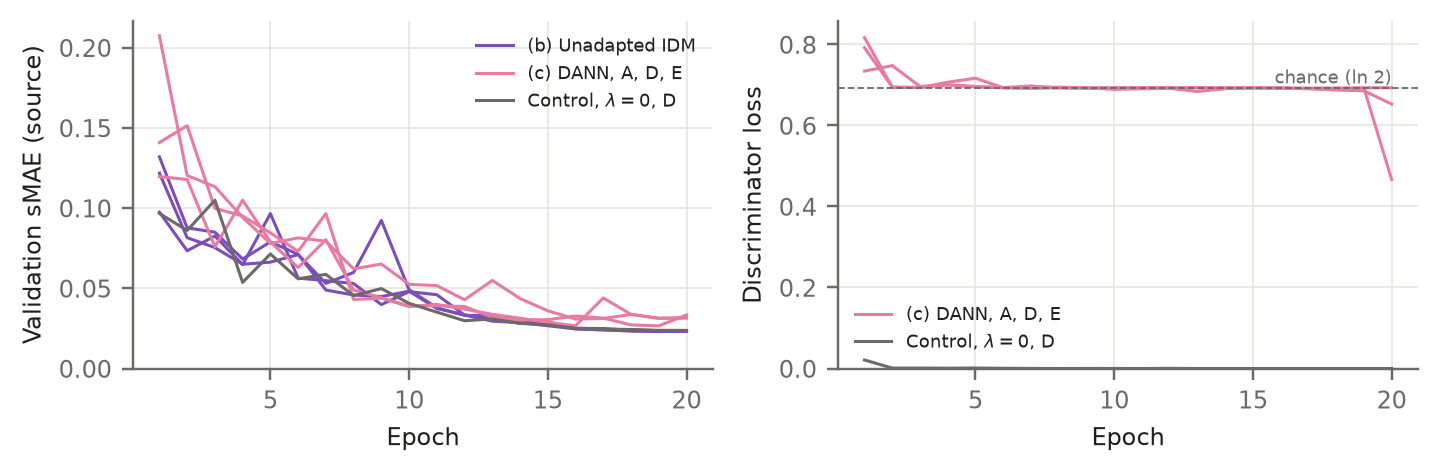
\includegraphics[width=0.9\linewidth]{../report/figures/dann_curves.png}

  \small Seed 0. DANN raises the source validation error (0.032 against 0.023); without the
  reversed gradient the discriminator separates the domains completely (loss near 0).
\end{frame}

\begin{frame}{Unadapted IDM (b), every seed}
  \centering
  \small
  \begin{tabular}{@{}llrrrr@{}}
    \toprule
    Target & Tested on & Seed 0 & Seed 1 & Seed 2 & Mean \\
    \midrule
    A & A / source & 63 / 88\% & 89 / 96\% & 97 / 94\% & 83.0 / 92.7\% \\
    D & D / source & 75 / 96\% & 80 / 94\% & 96 / 90\% & 83.7 / 93.3\% \\
    E & E / source & 98 / 43\% & 94 / 88\% & 93 / 82\% & 95.0 / 71.0\% \\
    E, no filter & E / source & 95 / 75\% & 97 / 98\% & 94 / 85\% & 95.3 / 86.0\% \\
    \bottomrule
  \end{tabular}

  \vspace{0.5em}
  Source success of the baseline: 90.7\%. R5 fails on E from seed 0 alone; without the
  filter it holds ($-4.7$ points), within the spread across seeds.
\end{frame}

\end{document}
